\section{Vektorrechner}

\begin{defi}[Vektorprozessoren]{Idee}
    Mathematisch-technische Anwendungen lassen sich erheblich in der Ausführung beschleunigen,
    wenn für Vektoroperationen:
    \begin{itemize}
        \item Spezielle, schnelle Hardware zur Verfügung steht und
        \item in der Programmiersprache Konstrukte zur Beschreibung von Vektor-Operationen verhanden sind
              (HPC Fortran, und zum Teil auch Fortran 90) oder
        \item der Compiler automatisch Programmteile als vektorisierbar erkennt
              (zum Teil mit Hilfe von Direktiven)
    \end{itemize}
    Mögliche Operationen (meist beschränkt auf Floating Point):
    \begin{itemize}
        \item $v = v \pm v, v = s \pm v$
        \item $v = v \cdot v, v = s \cdot v$
        \item mit n-elementigem Vektor $v$ und Skalar $s$
    \end{itemize}
    Eine Division wurde zunächst mit Hilfe einer Reziprok-Funktionseinheit berechnet:
    $v = \frac{1.0}{v}$
\end{defi}

\begin{defi}[Vektorprozessoren]{Ziel}
    Mit (im Idealfall!) einer Vektoroperation können gleichzeitig alle Elemente von zwei Vektoren verknüpft werden:
    \begin{align*}
        vc[1] & = va[1] \pm vb[1] \\
        \vdots                    \\
        vc[n] & = va[n] \pm vb[n]
    \end{align*}
    Dies braucht (im Idealfall!) für alle $n$ Elemente nicht mehr Rechenzyklen als die Berechnung für eine entsprechende Skalaroperation.
    Analog zum \enquote{Instruction Level Parallelism} (ILP) ist das Vector Processing eine Form des \enquote{Data Level Parallelism} (DLP).
\end{defi}

\begin{defi}{Data Level Parallelism (DLP)}\label{defi:dlp}
    \emph{Data Level Parallelism (DLP)} oder Datenparallelität ist die Parallelisierung über mehrere Prozessoren in parallelen Rechenumgebungen.
    Sie konzentriert sich auf die Verteilung der Daten auf verschiedene Knoten, die die Daten parallel bearbeiten.
    Sie kann auf reguläre Datenstrukturen wie Arrays und Matrizen angewendet werden, indem jedes Element parallel bearbeitet wird.
\end{defi}

\begin{defi}{Instruktions-Pipeline}

\end{defi}

\begin{defi}{Vektor-Pipeline}

\end{defi}

\section{Accelerators-Rechenbeschleuniger}

\begin{defi}{Aufbau CPU vs. GPU}
    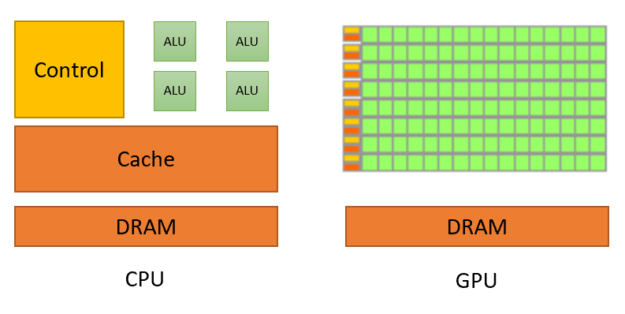
\includegraphics[width=\textwidth]{images/CPUvsGPU.png}
    Pradeep Gupta, CUDA Refresher: Reviewing the Origins of GPU Computing,
    \url{CUDA Refresher: Reviewing the Origins of GPU Computing},
    zuletzt aufgerufen am 17.06.2023 \\
    Mit \enquote{ALU} als \enquote{algorithmic logic unit} oder \enquote{arithmetisch-logische Einheit}.
\end{defi}

\subsection{Manycore-Architektur}

\begin{defi}{GPU}{Programmausführung}
    \begin{enumerate}
        \item Kopieren der Eingabedaten vom CPU Speicher in den DRAM der GPU.
        \item Laden und Ausführen des Programms auf der GPU, wobei Caching für eine bessere Performance genutzt wird.
        \item Kopieren der Ergebnisse vom DRAM der GPU zurück in den CPU Speicher.
    \end{enumerate}
\end{defi}

\begin{defi}{Field Programmable Gate Array (FPGA)}
    \begin{itemize}
        \item Integrierter Schaltkreis, der vom Anwender selbst (anwendungsspezifisch) konfiguriert werden kann.
        \item Enthält eine Vielzahl von Logikschaltungen wie AND, XOR (bis zu mehreren Millionen Gatter).
        \item Einzelne Komponenten können hierarchisch und beliebig miteinander verschaltet werden.
        \item Logikblöcke enthalten in der Regel Speicher-Blöcke (z.B. Flip-Flops).
        \item Können je nach Bauart mehrfach oder nur einmal programmiert werden (Schmelzbrücken).
    \end{itemize}
\end{defi}

\begin{defi}[Field Programmable Gate Array (FPGA)]{Anwendungen}
    \begin{itemize}
        \item Es existiert eine Hardware Description Language (HDL) zur Konfiguration eines FPGAs, wobei Tools wie z. B. HDL Coder von MathWorks verfügbar sind.
        \item Ermöglichen effizientes Lösen komplexer und sehr spezifischer Aufgaben.
        \item Können genutzt werden, um Chip-Design (ASIC) und Funktionalität vorab zu testen, bevor die implementierte Logik als Chip produziert wird.
        \item Eignen sich ebenfalls als Beschleuniger, z.B. in Kombination mit einer Host-CPU.
        \item Schnelle Anbindung über QPI (QuickPath Interconnect, Intel) oder über PCIe.
    \end{itemize}
\end{defi}

\section{Aufgaben}
